\section*{GBM}

Gradient Boosting Method is an agorithm that is part of \hyperref[sec:ensemble-methods]{ensemble methods}.

There are many different implementation of this algorithm; the below one (src: StatQuest) is one of the most generic and understandable.

\vspace{5mm}

1. Initialize model with constant value

$F_0 = \underset{\hat y}{argmin} ~\Sigma_{i=1}^n \mathcal{L}(y_i,\hat y)$

2. for $m = 1$ to $M$:

\hspace{1cm} (A) Compute pseudo-residuals:

\hspace{1cm} $r_{im} = - \frac{\partial \mathcal{L}(y_i, F(x_i))}{\partial F(x_i)}$ for $i=1,...,n$

\hspace{1cm} (B) Fit a weak learner with $r_m$ as target values

\hspace{1cm} (C) For $j=1,...,J_m$ (leafs) compute $\gamma_{jm} = \underset{\gamma}{argmin}~\Sigma_{x_i \in R_{ij}} \mathcal{L}(y_i, F_{m-1}(x_i)+\gamma)$

\hspace{1cm} (D) Update $F_m(x) = F_ {m-1}(x) + \alpha \Sigma_{j=1}^{J_m} \gamma_{jm} \mathbbm{1}(x \in R_{jm})$ for all records $x$

3. Output $F_M$

\vspace{5mm}

\underline{Step 1: initialize model with constant value}

$$F_0 = \underset{\hat y}{argmin} \Sigma_{i=1}^n \mathcal{L}(y_i,\hat y)$$

We note that $\hat y$ is constant and doesn't depend on $i$. Consequently, optimizing this equation using MSE will lead to $\hat y = \bar y$:

Note: $MSE := \frac{1}{n}\Sigma_{i=1}^n (y_i - \hat y)^2$ thus to use MSE in our case we need to have $\mathcal{L}: (y,\hat y) \to (y-\hat y)^2$ but we usually choose $\mathcal{L}: (y,\hat y) \to \frac{1}{2}(y-\hat y)^2$\\

$\frac{\partial MSE}{\partial \hat y} = 0$

=> $\frac{2}{n}(y_1 - \hat y) + ... + \frac{2}{n}(y_n - \hat y) = 0$

=> $\hat y = \Sigma_{i=1}^n \frac{y_i}{n} = \bar y$ \\

\underline{Step 2: loop on the number of estimators} \\

\textit{(A) Pseudo-residuals} \\

$$r_{im} = - \frac{\partial \mathcal{L}(y_i, F(x_i))}{\partial F(x_i)} \text{ for } i=1,...,n$$

The gradient of the loss function is $\frac{\partial \mathcal{L}}{\partial \hat y} = -(y - \hat y)$

Residuals as seen in linear regression are typically written as such: $res = y - \hat y$. Thus, gradient boosting uses negative residuals, also called \textbf{pseudo-residuals}. 

Note 1: pseudo-residuals are just the derivatives of the loss function; that's why we call it \textbf{gradient} boosting.

Note 2: $F(x_i)$ is the prediction of each record that is equivalent to $\hat y$.

\textit{Reminder}:  the prediction of a decison tree is found in navigating from the root to the leaf where the sample is classified.  \\

\textit{(B) Fit a weak learner with $r_m$ as target values} \\

\lstset{language=Python}
\lstset{frame=lines}
\lstset{caption={Fit base learner}}
\lstset{label={lst:code_direct}}
\lstset{basicstyle=\footnotesize}
\begin{lstlisting}
h = tree.fit(x, res)
\end{lstlisting}

Weak learners (see definition in \hyperref[sec:adaboost]{Adaboost} section) used in gradient boosting are typically decision trees. These learners are trained on residuals. 

Thus, this step consists in building a small tree. \\

\textit{(C) Compute a unique output for each leaf} \\

We could call this step: "harmonization of predicted values". \\

For $j=1,...,J_m$:

$$\gamma_{jm} = \underset{\gamma}{argmin}~\Sigma_{x_i \in R_{ij}} \mathcal{L}(y_i, F_{m-1}(x_i)+\gamma)$$

The loop "For $j=1,...,J_m$" means we iterate on all leafs of the previously built tree.

This step consists in building a unique output for each of its leaf. $R_{j,m}$ are the terminal regions, that is, the leafs of the tree. \\

In the below picture the first weak learner is shown. Here $J_m=2$ since there are 2 leafs only.

We also consider the MSE as a loss function, so $\gamma_{jm}$ is equal to the averages of the leaf outputs.

\begin{center}
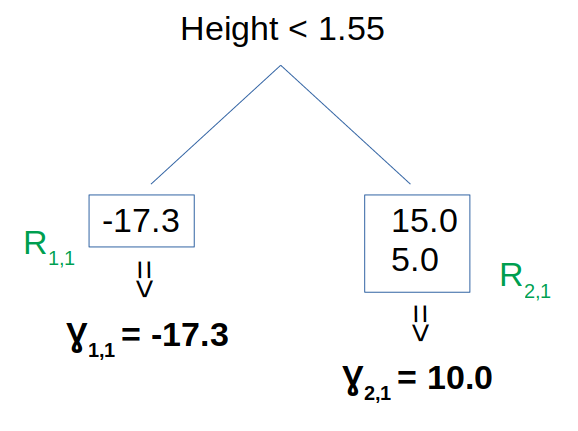
\includegraphics[scale=0.3]{GBM_regression_leafs.png}
\end{center}

\textit{(D) Update the function} \\

$$F_m(x) = F_ {m-1}(x) + \alpha \Sigma_{j=1}^{J_m} \gamma_{jm} \mathbbm{1}(x \in R_{jm})$$

$\alpha$ is the \textit{learning rate} used to reduce overfitting.

The summation is here only in case one record $x$ ends up in several leafs.\\

\underline{Step 3: Output the function} \\

$F$ is the output of the algorithm and is just a combination of several trees. To find the predicted value of a record, we would need to sum all predicted values of each tree (weighted by the learning rate $\alpha$). Below is an illustration of the computation of the final prediction for a record $x$:

\begin{center}
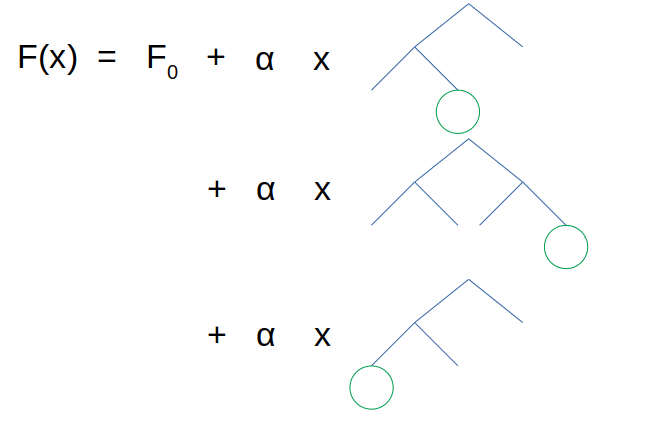
\includegraphics[scale=0.3]{GBM_final_function.png}
\end{center}

\vspace{5mm}